
%%%%%%%%%%%%%%%%%%%%%%%%%%%%% Thesis.tex %%%%%%%%%%%%%%%%%%%%%%%%%%%%%%%
%                                                                      %
%  ---------- Master of Science Dissertation template ----------       %
%                                                                      %
%  Template for the Master Thesis according to the regulations         %
%  published by the Scientific Council at IST.                         %
%                                                                      %
%  For up-to-date regulations, please refer to                         %
%  http://cd.ist.utl.pt/files/publico/academicos/guia_dissertacao.pdf  %
%                                                                      %
%       Email: caar@ist.utl.pt                                  %
%                                                                      %
%  Created:       Jan 20, 2011                                         %
%  Last Modified: Oct 30, 2012                                         %
%                                                                      %
%%%%%%%%%%%%%%%%%%%%%%%%%%%%%%%%%%%%%%%%%%%%%%%%%%%%%%%%%%%%%%%%%%%%%%%%
%  Revision history                                                    %
%  v1 - 2011/01/24 - original template                                 %
%  v2 - 2012/10/30 - new IST image and glossary support                %
%%%%%%%%%%%%%%%%%%%%%%%%%%%%%%%%%%%%%%%%%%%%%%%%%%%%%%%%%%%%%%%%%%%%%%%%
%                                                                      %
% To generate the PDF file, type "make" at the terminal prompt.        %
%                                                                      %
% The IST template LaTeX package was created by the author             %
% and it can be downloaded from:                                       %
% https://fenix.ist.utl.pt/homepage/ist31052/                          %
%                                                                      %
% The external packages can be downloaded from                         %
% the Comprehensive TeX Archive Network at http://www.ctan.org/        %
%                                                                      %
% List of LaTex symbols:                                               %
% http://www.ctan.org/tex-archive/info/symbols/comprehensive/          %
%                                                                      %
% Help with LaTex can be found at                                      %
% http://www.giss.nasa.gov/tools/latex/ltx-2.html                      %
% http://en.wikibooks.org/wiki/LaTeX                                   %
%%%%%%%%%%%%%%%%%%%%%%%%%%%%%%%%%%%%%%%%%%%%%%%%%%%%%%%%%%%%%%%%%%%%%%%%

%%%%%%%%%%%%%%%%%%%%%%%%%%%%%%%%%%%%%%%%%%%%%%%%%%%%%%%%%%%%%%%%%%%%%%%%
%     Preamble                                                         %
%%%%%%%%%%%%%%%%%%%%%%%%%%%%%%%%%%%%%%%%%%%%%%%%%%%%%%%%%%%%%%%%%%%%%%%%

% ----------------------------------------------------------------------
%  Set the document class
% ----------------------------------------------------------------------
\documentclass[10pt,a4paper,twoside]{report}

% ----------------------------------------------------------------------
% Define external packages, language, margins, fonts and new commands
% ----------------------------------------------------------------------
\input{Thesis_Preamble} % file "Thesis_Preamble.tex"
%%%%%%%%%%%%%%%%%%%%%%%%%%%%%%%%%%%%%%%%%%%%%%%%%%%%%%%%%%%%%%%%%%%%%%%%
%     Begin Document                                                   %
%%%%%%%%%%%%%%%%%%%%%%%%%%%%%%%%%%%%%%%%%%%%%%%%%%%%%%%%%%%%%%%%%%%%%%%%
\begin{document}

% Set plain page style (no headers, footer with centered page number)
\pagestyle{plain}

% Set roman numbering (i,ii,...) before the start of chapters
\pagenumbering{roman}

% ----------------------------------------------------------------------
%  Cover page
% ----------------------------------------------------------------------
%%%%%%%%%%%%%%%%%%%%%%%%%%%%%%%%%%%%%%%%%%%%%%%%%%%%%%%%%%%%%%%%%%%%%%%%
%                                                                      %
%     File: Thesis_FrontCover.tex                                      %
%     Tex Master: Thesis.tex                                           %
%                                                                      %
%     Author: Andre C. Marta                                           %
%     Last modified :  2 Jul 2015                                      %
%                                                                      %
%%%%%%%%%%%%%%%%%%%%%%%%%%%%%%%%%%%%%%%%%%%%%%%%%%%%%%%%%%%%%%%%%%%%%%%%

\thispagestyle {empty}

% IST Logo - Signature A
% parameters: bb=llx lly urx ury (bounding box), width=h_length, height=v_length, angle=angle, scale=factor, clip=true/false, draft=true/false. 
\includegraphics[bb=9.5cm 11cm 0cm 0cm,scale=0.29]{IST_A_CMYK_POS}

\begin{center}
%
% Title, author and degree
\vspace{3.0cm}
{\FontLb Simulator for the Versat Reconfigurable Processor} \\ % <<<<< EDIT TITLE
%\vspace{0.2cm}
%{\FontMn Subtitle (optional)} \\
%\vspace{1.9cm}
\vspace{2.6cm}
{\FontMb João César Martins Moutoso Ratinho} \\ % <<<<< EDIT NAME
\vspace{2.0cm}
{\FontSn \coverThesis} \\
\vspace{0.3cm}
{\FontLb Electrical and Computer Engineering} \\ % <<<<< EDIT COURSE
\vspace{1.0cm}
{\FontSn %
\begin{tabular}{ll}
 \coverSupervisors: & Prof. José João Henriques Teixeira de Sousa \\ % <<<<< EDIT NAME
 
\end{tabular} } \\
\vspace{1.0cm}
{\FontMb \coverExaminationCommittee} \\
\vspace{0.3cm}
{\FontSn %
\begin{tabular}{c}
%\coverChairperson:     Prof. Gonçalo Nuno Gomes Tavares          \\ % <<<<< EDIT NAME
\coverSupervisor:      Prof. José João Henriques Teixeira de Sousa \\ % <<<<< EDIT NAME
Member of the Committee: Prof. Marcelino Bicho dos Santos          % <<<<< EDIT NAME
\end{tabular} } \\
\vspace{1.5cm}
{\FontMb January 2019} \\ % <<<<< EDIT DATE (corresponds to date of oral examination)
%
\end{center}

 % file "Thesis_FrontCover.tex"

% ----------------------------------------------------------------------
% Dedication page (optional)
% ----------------------------------------------------------------------
%%%%%%%%%%%%%%%%%%%%%%%%%%%%%%%%%%%%%%%%%%%%%%%%%%%%%%%%%%%%%%%%%%%%%%%%
%                                                                      %
%     File: Thesis_Dedication.tex                                      %
%     Tex Master: Thesis.tex                                           %
%                                                                      %
%     Author: Gonçalo Santos                                           %
%     Last modified : 20 Oct 2018                                      %
%                                                                      %
%%%%%%%%%%%%%%%%%%%%%%%%%%%%%%%%%%%%%%%%%%%%%%%%%%%%%%%%%%%%%%%%%%%%%%%%

%\null\vskip5cm%
%\begin{flushright}
%     Dedicated to someone special...
%\end{flushright}
%\vfill\newpage

\section*{Declaration}
I declare that this document is an original work of my own authorship
and that it fulfills all the requirements of the Code of Conduct and
Good Practices of the Universidade de Lisboa.

\cleardoublepage

 % file "Thesis_Dedication.tex"

% ----------------------------------------------------------------------
%  Acknowledgments (optional)
% ----------------------------------------------------------------------
%%%%%%%%%%%%%%%%%%%%%%%%%%%%%%%%%%%%%%%%%%%%%%%%%%%%%%%%%%%%%%%%%%%%%%%%
%                                                                      %
%     File: Thesis_Acknowledgments.tex                                 %
%     Tex Master: Thesis.tex                                           %
%                                                                      %
%     Author: Andre C. Marta                                           %
%     Last modified :  2 Jul 2015                                      %
%                                                                      %
%%%%%%%%%%%%%%%%%%%%%%%%%%%%%%%%%%%%%%%%%%%%%%%%%%%%%%%%%%%%%%%%%%%%%%%%

\section*{\acknowledgments}

% Add entry in the table of contents as section
\addcontentsline{toc}{section}{\acknowledgments}

I want to thank my supervisor, Professor José Teixeira de Sousa, for the 
opportunity to develop this work and for his guidance and support during that process. 
His help was fundamental to overcome the multiple obstacles that I faced during this work.

I also want to acknowledge Professor Horácio Neto for providing a simple Convolutional 
Neural Network application, used as a basis for the application developed for the 
RV32-Versat architecture.

A special acknowledgement goes to my friends, for their continuous support, and Válter,  
that is developing a multi-layer architecture for RV32-Versat. When everything seemed to 
be doomed he always had a miraculous solution.

Finally, I want to express my sincere gratitude to my family for giving me all the 
support and encouragement that I needed throughout my years of study and through the 
process of researching and writing this thesis. They are also part of this work.\\

\textbf{Thank you.}

 % file "Thesis_Acknowledgements.tex"

% ----------------------------------------------------------------------
%  Abstract (both in English and Portuguese)
% ----------------------------------------------------------------------
%%%%%%%%%%%%%%%%%%%%%%%%%%%%%%%%%%%%%%%%%%%%%%%%%%%%%%%%%%%%%%%%%%%%%%%%
%                                                                      %
%     File: Thesis_Resumo.tex                                          %
%     Tex Master: Thesis.tex                                           %
%                                                                      %
%     Author: João D. Lopes                                            %
%     Last modified :  15 October 2017                                 %
%                                                                      %
%%%%%%%%%%%%%%%%%%%%%%%%%%%%%%%%%%%%%%%%%%%%%%%%%%%%%%%%%%%%%%%%%%%%%%%%

\section*{Resumo}

% Add entry in the table of contents as section
\addcontentsline{toc}{section}{Resumo}

Esta tese descreve o Versat, um acelerador de hardware reconfigurável
para sistemas embebidos. O Versat é uma arquitetura de matriz
reconfigurável de grão grosso e de baixa potência, que implementa
reconfiguração auto-gerada e parcial usando um controlador. Esta
abordagem visa aplicações de muito baixo consumo energético, como as
encontradas em redes de sensores sem fios, onde o uso de GPUs ou FPGAs
está fora de questão. Comparado com outras arquitecturas, o Versat
possui um baixo número de unidades funcionais interligadas em
topologia de grafo completo. O número de unidades funcionais é
compensado pela facilidade de configuração e reconfiguração. Ao
contrário de outras arquitecturas, o Versat pode mapear sequências de
malhas aninhadas em vez de uma única malha; a reconfiguração
auto-gerada e parcial ocorre entre malhas aninhadas. O Versat pode ser
programado em assembly ou em C++. A programação em assembly é uma
característica útil para optimização de programas e contorno de erros
de compilação/arquitetura. Este trabalho contribuiu para o projecto de
todo o sistema, com especial ênfase nas fases de verificação,
depuração, restrições temporais, concorrência ao nível de circuito de
dados, acesso directo à memória, interfaces AXI, programas para
caracterização e testes de regressão. Resultados de caracterização
mostram que o Versat pode acelerar algoritmos de configuração única
até 4x com um consumo energético uma ordem de grandeza inferior
comparado com um processador de referência. No caso de algoritmos com
múltiplas configurações, os benefícios são ainda maiores: aceleração
de 20x com até 2 ordens de grandeza de mais eficiência energética.

\vfill

\textbf{\Large Palavras-chave:} Computação reconfigur{\'a}vel, Matrizes Reconfigur{\'a}veis de Gr{\~a}o Grosso, Sistemas Embebidos, Sistemas de Baixa Pot{\^e}ncia


 % file "Thesis_Resumo.tex"
%%%%%%%%%%%%%%%%%%%%%%%%%%%%%%%%%%%%%%%%%%%%%%%%%%%%%%%%%%%%%%%%%%%%%%%%
%                                                                      %
%     File: Thesis_Abstract.tex                                        %
%     Tex Master: Thesis.tex                                           %
%                                                                      %
%     Author: João D. Lopes                                            %
%     Last modified :  18 May 2016                                     %
%                                                                      %
%%%%%%%%%%%%%%%%%%%%%%%%%%%%%%%%%%%%%%%%%%%%%%%%%%%%%%%%%%%%%%%%%%%%%%%%

\section*{Abstract}

% Add entry in the table of contents as section
\addcontentsline{toc}{section}{Abstract}

This report introduces Versat, a reconfigurable hardware accelerator
to be used in an embedded system in order to optimize performance and
power. Versat is a Coarse-Grain Reconfigurable Array architecture
(CGRA), which implements self and partial reconfiguration by using a
simple controller unit. Compared to other CGRAs, Versat has a smaller
number of functional units with a fully connected graph topology for
maximum flexibility. The idea is to operate in a region of the design
space, where less computations can be mapped onto the array but the
array itself is more frequently reconfigured. An original feature of
Versat is the ability to map sequences of nested program loops instead
of just one program loop. Reconfiguration happens when moving from one
nested loop to the next. Experimental results are presented.

\vfill

\textbf{\Large Keywords:} reconfigurable computing, coarse-grain reconfigurable arrays, embedded systems

 % file "Thesis_Abstract.tex"

% ----------------------------------------------------------------------
%  Table of contents, list of tables, list of figures and nomenclature
% ----------------------------------------------------------------------

% Table of contents
%
\tableofcontents
\cleardoublepage 

% List of tables
%
% Generate list
\listoftables
% Add entry in the table of contents as section
\addcontentsline{toc}{section}{\listtablename}
\cleardoublepage 

% List of figures
%
% Generate list
\listoffigures
% Add entry in the table of contents as section
\addcontentsline{toc}{section}{\listfigurename}
\cleardoublepage 

%% Nomenclature
%%
%% entries of nomenclature list
%\input{Thesis_Nomenclature} % file "Thesis_Nomenclature.tex"
%%
%% Insert glossary/nomenclature section produced by MakeIndex
%\printnomenclature
%% Add entry in the table of contents as section
%\addcontentsline{toc}{section}{\nomname}
%\cleardoublepage

% entries of glossary list
%%%%%%%%%%%%%%%%%%%%%%%%%%%%%%%%%%%%%%%%%%%%%%%%%%%%%%%%%%%%%%%%%%%%%%%%%
%                                                                      %
%     File: Thesis_Glossary.tex                                        %
%     Tex Master: Thesis.tex                                           %
%                                                                      %
%     Author: Carlos A. Rodrigues                                           %
%     Last modified : 30 Oct 2012                                      %
%                                                                      %
%%%%%%%%%%%%%%%%%%%%%%%%%%%%%%%%%%%%%%%%%%%%%%%%%%%%%%%%%%%%%%%%%%%%%%%%
%
% The definitions can be placed anywhere in the document body
% and their order is sorted by <symbol> automatically when
% calling makeindex in the makefile
%
% The \glossary command has the following syntax:
%
% \glossary{entry}
%
% The \nomenclature command has the following syntax:
%
% \nomenclature[<prefix>]{<symbol>}{<description>}
%
% where <prefix> is used for fine tuning the sort order,
% <symbol> is the symbol to be described, and <description> is
% the actual description.

% ----------------------------------------------------------------------

\glossary{name={\textbf{OpenOCD}},description={Open On-Chip Debugger}}

\glossary{name={\textbf{JTAG}},description={joint Test Action Group}}

\glossary{name={\textbf{SCLK}},description={Serial Clock, linha de clock.}}

\glossary{name={\textbf{MOSI}},description={Master Output Slave Input, saida no mestre entrada no escravo .}}

\glossary{name={\textbf{MISO}},description={Master Input Slave Output, entrada no mestre saida no escravo .}}

\glossary{name={\textbf{SS}},description={Slave Select, Escolha de escravo.}}

\glossary{name={\textbf{SDA}},description={Serial Data Line, linha serie de dados .}}

\glossary{name={\textbf{SCL}},description={Serial Clock Line. linha serie de clock}}



 % file "Thesis_Glossary.tex"

% Insert glossary section produced by MakeIndex
%\printglossary
% Add entry in the table of contents as section
%\addcontentsline{toc}{section}{\glossaryname}
%\cleardoublepage

%acronimos mudar todos os acronimos para o formato como esta o ACK

\vspace*{1.95cm} \hspace*{-0.5cm} %,88
\textbf{{\huge \sffamily Lista de Acrônimos}\\}
\vspace*{0.5cm}
\begin{acronym}
\addcontentsline{toc}{chapter}{Lista de Acrônimos}
\thispagestyle{plain}
\setcounter{page}{13}
\newacronym{soc}{SoC}{\textit{System on Chip}}
\newacronym{uart}{UART}{\textit{Universal Asynchronous Receiver/Transmitter}}
\newacronym{gpio}{GPIO}{\textit{General Purpose Input/Output}}
\newacronym{risc}{RISC}{\textit{Reduced Instruction Set Computing}}
\newacronym{or1200}{OR1200}{\textit{OpenRISC12000}}
\newacronym{fpga}{FPGA}{\textit{Field Programmable Gate Array}}
\newacronym{jtag}{JTAG}{\textit{Joint Test Action Group}}
\newacronym{orpsoc}{ORPSoC}{\textit{OpenRISC Reference Platform System-on-Chip}}
\newacronym{ads}{ADS}{\textit{Advenced Debug System}}
\newacronym{usb}{USB}{\textit{Universal Serial Bus}}
\newacronym{openocd}{OpenOCD}{\textit{Open On-Chip Degugger}}
\newacronym{rsp}{RSP}{\textit{Remote Serial Protocol}}
\newacronym{bios}{BIOS}{\textit{Basic Input Output System}}
\newacronym{fifo}{FIFO}{\textit{Frist In First Out}}
\newacronym{i2c}{I2C}{\textit{Inter-Integrated Circuit}}
\newacronym{scl}{SCL}{\textit{Serial Clock}}
\newacronym{sda}{SDA}{\textit{Serial Data}}
\newacronym{spi}{SPI}{\textit{Serial Peripheral Interface}}
\newacronym{sclk}{SCLK}{\textit{Serial Clock}}
\newacronym{mosi}{MOSI}{\textit{Master Out Slave In}}
\newacronym{miso}{MISO}{\textit{Master In Slave Out}}
\newacronym{ss}{SS}{\textit{Slave Select}}
\newacronym{sd}{SD}{\textit{Security Digital}}
\acro{ACK}{Acknowledge}
\end{acronym}
\cleardoublepage
% Set arabic numbering (1,2,...) after preface
%
\setcounter{page}{1}
\pagenumbering{arabic}

% ----------------------------------------------------------------------
%  Chapters
% ----------------------------------------------------------------------

%%%%%%%%%%%%%%%%%%%%%%%%%%%%%%%%%%%%%%%%%%%%%%%%%%%%%%%%%%%%%%%%%%%%%%%%
%                                                                      %
%     File: Thesis_Introduction.tex                                    %
%     Tex Master: Thesis.tex                                           %
%                                                                      %
%     Author: João D. Lopes                                            %
%     Last modified :  2 June 2016                                     %
%                                                                      %
%%%%%%%%%%%%%%%%%%%%%%%%%%%%%%%%%%%%%%%%%%%%%%%%%%%%%%%%%%%%%%%%%%%%%%%%

\chapter{Introduction}
\label{chapter:introduction}

\section{Motivation}
\label{section:motivation}

With the expansion in the number of features, modern embedded systems
are becoming more and more power hungry. Therefore it is crucial to
minimize power consumption. The main reason for this low power demand
is the short battery life of most devices used daily.

Another problem is the device price. The smaller the circuit the
cheaper it will be, and higher profit margins can be obtained from
it. Therefore, if one can deliver the same functionality with a
smaller and more power efficient device, one will have a more
competitive product.

These problems have been tackled with smaller and smaller transistors
which can work at higher frequencies without changing the
architecture. However, with the eminent demise of Moore's law and the
advent of the Internet of Things (IoT), this solution is not
viable. Reconfigurable hardware, which is known to be extremely
efficient in terms of power consumption and silicon area utilization,
has been used in mid-range to high-end applications. Fine grain
reconfigurable fabrics such as Field-Programmable Gate Arrays (FPGAs)
can be an alternative but, compared to Coarse-Grain Reconfigurable Arrays
(CGRAs), embedded FPGA cores consume significantly more silicon area and
power.

A CGRA is a collection of programmable functional units and embedded
memories connected by programmable interconnects. This structure is
what is called the reconfigurable array. When given a set of
configuration bits, the reconfigurable array forms a hardware datapath
able to execute a certain task orders of magnitude faster than a
conventional Central Processing Unit (CPU). CGRAs are used as hardware
co-processors to accelerate algorithms that are time/power consuming in
regular CPUs.

Normally, the reconfigurable array is used only to accelerate program
loops and the non-loop code is run on an attached processor which has
a conventional architecture. For this reason, CGRAs normally include a
conventional processor. For example, the Morphosys
architecture~\cite{Lee00} integrates a small Reduced Instruction Set
Computer (RISC) and the ADRES architecture~\cite{Mei05} integrates a
Very Large Instruction Word (VLIW) processor.


\section{Problems addressed}
\label{section:problemsAddressed}

The main problems that we have identified with existing CGRAs are
their large size, limited reconfiguration control and difficulty
in programming. Therefore, we propose some architectural improvements
to address these problems which follow three basic ideas.

The first idea is to make the CGRA smaller and to use fully connected
graph topology. Normally, graphs with constrained connectivity are
employed in CGRAs to avoid decreasing the frequency of
operation. However, low power devices will rarely choose to operate at
a high frequency, so using a fully connected graph becomes a
possibility. In terms of silicon area, fewer compute nodes can be used
if all nodes are connected to one another but more routing resources
are needed. Fortunately, these routing resources do not increase power
consumption as our reconfiguration frequency is low. In fact, our
reconfiguration process is more frequent compared to static arrays
such as~\cite{Hartenstein99}, but much less frequent compared to
dynamic arrays such as~\cite{Mei05}. Although we cannot build large
datapaths with many functional units, because we use fewer, we can
build {\it any} datapath with the functional units we do have.
Finally, programming is drastically simplified as there is no need for
{\em place \& route} algorithms in the compilation flow such as in
FPGAs and other fabrics.

The second idea is to make the configuration register addressable to
the word level. The configuration is divided in spaces, which
correspond to each functional unit, and the configuration spaces are
further divided in configuration fields which are made individually
addressable. Partial reconfiguration is useful to keep reconfiguration
to a minimum, exploiting the similarity between successive
configurations. Reducing reconfiguration time has a dramatic influence
on improving the performance, which can compensate for a lower
frequency of operation.

The third idea is to integrate a specialized and programmable
controller in the CGRA to manage reconfigurations and data transfers
to/from external memory. The controller is in charge of the main
program flow of the accelerator, sequencing the configurations and
using partial reconfiguration whenever possible. The controller can
spawn data stream compute threads in the CGRA and data movement
threads using a Direct Memory Access (DMA) unit. While these threads are
running, the controller can prepare the next configurations.


\begin{comment}

Normally, the reconfigurable array is used only to accelerate program
loops and the non-loop code is run on an attached processor which has
a conventional architecture. For this reason, CGRAs normally include a
conventional processor. For example, the Morphosys
architecture~\cite{Lee00} integrates a small Reduced Instruction Set
Computer (RISC) and the ADRES architecture~\cite{Mei05} integrates a
Very Large Instruction Word (VLIW) processor.

\end{comment}

%Relevance of the subject...


%%%%%%%%%%%%%%%%%%%%%%%%%%%%%%%%%%%%%%%%%%%%%%%%%%%%%%%%%%%%%%%%%%%%%%%%
\section{Topic Overview}
\label{section:overview}

In this work we presente Versat, a new reconfigurable hardware
accelerator which is suitable for low-cost low-power devices. Its
architecture uses a relatively small number of functional units and a
simple controller. A smaller array limits the size of the data
expressions that can be mapped to the CGRA but large expressions can
be broken into smaller expressions which can be executed sequentially
in the CGRA. Therefore, Versat requires mechanisms for handling large
numbers of configurations and frequent reconfigurations efficiently.

Versat is to be used as a co-processor featuring an Application Programming
Interface (API) containing a set of useful kernels. Applications developers
can use a commercial embedded processor with a rich ecosystem and drop in a
Versat core for performance and power optimization. Versat programmers can
create a set of useful kernels that application programmers will want to
use. In this way, the software and programming tools of the CGRA are
clearly separated from those of the application processor. This makes
Versat suitable for supporting the Open Computing Language (OpenCL)
standard or others.

%Provide an overview of the topic to be studied...


%%%%%%%%%%%%%%%%%%%%%%%%%%%%%%%%%%%%%%%%%%%%%%%%%%%%%%%%%%%%%%%%%%%%%%%%
\section{Objectives}
\label{section:objectives}

The main objective of this new architecture is to get acceleration
with low power consumption and small silicon area.

In fact, Versat can replace a number of dedicated hardware
accelerators in a System on Chip (SoC), making it smaller, more power
efficient and safer to design (the development risk of designing
dedicated hardware accelerators is eliminated).

Digital signal processing applications are targeted: biometrics,
speech recognition, artificial vision, security, etc. The overall goal
of the project is to create an Intellectual Property (IP) core and a
library of useful procedures. A clean procedural interface to a host
becomes possible. With such an interface the host can have tasks
executed in the CGRA by simply calling procedures and passing
arguments.

%Explicitly state the objectives set to be achieved with this thesis...

%%%%%%%%%%%%%%%%%%%%%%%%%%%%%%%%%%%%%%%%%%%%%%%%%%%%%%%%%%%%%%%%%%%%%%%%
\section{Author's Work}
\label{section:authorWork}

%falar no trabalho feito por outros; trabalho feito pelo autor
The work presented here is the result of the work of a few
people. When I started working on this project, in the summer of 2014,
there was a preliminary, non-functional version of the system.  I
contributed the multi-threading idea, where the state machines of the
address generators work independently, I pipelined parts of the
implementation to improve the frequency of operation, I wrote the boot
Read Only Memory (ROM) software and its hand shaking protocol with a
host system. I also implemented the DMA design, master and slave
Advanced Extensible Interface (AXI) interfaces, contributed to the
Application-Specific Integrated Circuit (ASIC) implementation, and,
finally, I wrote all assembly kernels used for tests and implemented a
regression test system where it is easy to add or remove new tests. As
a result of this work, the team has already a paper accepted for
publication~\cite{deSousa16}.

%%%%%%%%%%%%%%%%%%%%%%%%%%%%%%%%%%%%%%%%%%%%%%%%%%%%%%%%%%%%%%%%%%%%%%%%
\section{Report Outline}
\label{section:outline}

This report is composed by a few more chapters. In the second chapter,
the advantages and disadvantages of other architectures are
discussed. In the third chapter, Versat's architecture is fully
described. In the fourth chapter, some experimental results are
presented. In the fifth and final chapter, our achievements are
pointed out and some future work is outlined.

%Briefly explain the contents of the different chapters...

 % file "Thesis_Introduction.tex"

\chapter{Estado-da-arte}
\label{chapter:estadodaarte}

\section{OpenRisc}
\label{section:OpenRisc}

é uma comunidade opensource que desenvolve hardware e ferramentas que ajudam a na cria\c{c}\~ao de novos sistemas o OrpSoc

cores têm codigo escrito verilog e VDH sendo o verilog maioritário

\subsection{Toolchain}

é a toolchain da GNU onde foi adicionado o processador desenvolvida pela comunidade.

foi desenvolvida pela comunidade falar sobre ferramenteas 

tem a selac\c{c}\~ao do de onde o codigo vais correr.

por uma imagem a explicar a ideia de ser preciso compilar com o mboard

\subsection{OrpSoc}

explicar a ferramente que foi desenvolvida para que serve e as vantagens 

mudou de nome (FuseSoc)para se tornar uma ferramente independente da comunidade.

por uma imagem de como o OrpSoc está construido.

\section{Ferramentas de simula\c{c}\~ao}
\label{section:ferramentas}

vantagem de ter um sistema de simula\c{c}\~ao.

\subsection{Or1ksim}

dizer que é um simulador desenvolvido em C que predente simular o processador.

vantagens e desvantagens

\subsection{Icarus}

explicar como funciona o icarus que precisa de uma testbench em verilog, dá para ver as ondas e tem a vantagem de ter o estado de alta impedancia. 

Mas demora muito tempo.

Por uma imagem das ondas com alta impedancia com um tempo igual no verilog

\subsection{Verilator}

explica como funciona o verilator, converte os codigo em verilog em codigo C ou systemC conforme o que a pessoa pretender.

pode ser a testbench escrita em C ou systemC, que se pode ver as ondas e têm a desvantagem que n\~ao conseguir sumilar o estado de alta impetancia.

muito rapido comparado com o icarus

Por uma imagem das ondas com alta impedancia com um tempo igual no icarus

\subsection{Placa FPGA}

explicar o que é como funciona 

como funciona

\section{OpenOCD}
\label{section:OpenOCD}

explicar para que server e como é ligado. e as portas para cada ferramenta.

Por uma imagem sobre como é ligado o openocd

\section{Protocolos}
\label{section:protocolos}

\subsection{Uart}

falar da uart como funciona o protocolo

\subsection{GPIO}

falar um pouco do GPIO como funciona

\subsection{I2C}

Falar do I2C como funciona os pinos que tem para que servem

falar e imagem so start, stop bit e dos dados

\subsection{SPI}

falar do SPI. como funcionar quais s\~ao os pinos que tem. para que serve cada um
 % file "Thesis_Estado_da_arte.tex"

%%%%%%%%%%%%%%%%%%%%%%%%%%%%%%%%%%%%%%%%%%%%%%%%%%%%%%%%%%%%%%%%%%%%%%%%
%                                                                      %
%     File: Thesis_SPI.tex                        %
%     Tex Master: Thesis.tex                                %
%                                                                      %
%     Author: Carlos A. Rodrigues                         %
%     Last modified : 15 Abril 2013                         %
%                                                                      %
%%%%%%%%%%%%%%%%%%%%%%%%%%%%%%%%%%%%%%%%%%%%%%%%%%%%%%%%%%%%%%%%%%%%%%%

\chapter{SPI}
\label{chapter:spi}


Explicar o protocolo spi. como funciona e as linhas que tem. explicar em que casos \'e mais usado

por uma imagem os um master e slaves para mostrar como s\~ao as liga\c{c}\~oes

\section{Mestre SPI}

estado do core.  dizer que o master spi s\'o conseguia enviar e nao recebia qualquer tipo de informa\c{c}\~ao

por um diagrama de blocos de como circula a informa\c{c}\~ao dentro do meu modelo de SPI. fazer uma descri\c{c}\~ao do funcionamento com uma descri\c{c}ao do fluxo de dados.

por a tabela de sinais da interface de SPI (sinais de entrada e saida)

tabela de registos (endere\c{c}os do registos).

explicar os 2 modos de funcionamento de esrita e de leitura que tem 2 modos.

\section{escravo SPI}

dizer que foi desenhado desde o inicio.

por um diagrama de blocos de como circula a informa\c{c}\~ao dentro do meu modelo de SPI. fazer uma descri\c{c}\~ao do funcionamento com uma descri\c{c}ao do fluxo de dados.

por a tabela de sinais da interface de SPI (sinais de entrada e saida)

tabela de registos (endere\c{c}os do registos).

explicar os 2 modos de funcionamento de esrita e de leitura que tem 2 modos.
 % Thesis_Spi.tex

%%%%%%%%%%%%%%%%%%%%%%%%%%%%%%%%%%%%%%%%%%%%%%%%%%%%%%%%%%%%%%%%%%%%%%%%
%                                                                      %
%     File: Thesis_I2C.tex                        %
%     Tex Master: Thesis.tex                                %
%                                                                      %
%     Author: Carlos A. Rodrigues                         %
%     Last modified : 15 Abril 2013                         %
%                                                                      %
%%%%%%%%%%%%%%%%%%%%%%%%%%%%%%%%%%%%%%%%%%%%%%%%%%%%%%%%%%%%%%%%%%%%%%%

\chapter{I2C}
\label{chapter:i2c}


Explicar o protocolo i2c. como funciona e as linhas que tem. explicar em que acasos é mais usado

por uma imagem os um master e slaves para mostrar como s\~ao as liga\c{c}ões

\section{Mestre I2C}

dizer como estava o master a I2C que n\~ao conseguia enviar ao receber dados.

por um diagrama de blocos de como circula a informa\c{c}\~ao dentro do meu modelo de SPI. fazer uma descri\c{c}\~ao do funcionamento com uma descri\c{c}ao do fluxo de dados.

por a tabela de sinais da interface de i2c (sinais de entrada e saida)

tabela de registos (endere\c{c}os do registos).

explicar os 2 modos de funcionamento de esrita e de leitura que tem 2 modos.

\section{escravo I2C}

processo de constru\c{c}\~ao do escravo 

por um diagrama de blocos de como circula a informa\c{c}\~ao dentro do meu modelo de SPI. fazer uma descri\c{c}\~ao do funcionamento com uma descri\c{c}ao do fluxo de dados.

por a tabela de sinais da interface de i2c (sinais de entrada e saida)

tabela de registos (endere\c{c}os do registos).

explicar os 2 modos de funcionamento de esrita e de leitura que tem 2 modos.
 % Thesis_I2C.tex

%%%%%%%%%%%%%%%%%%%%%%%%%%%%%%%%%%%%%%%%%%%%%%%%%%%%%%%%%%%%%%%%%%%%%%%%
%                                                                      %
%     File: Thesis_Interface_FIFO.tex                        %
%     Tex Master: Thesis.tex                                %
%                                                                      %
%     Author: Carlos A. Rodrigues                         %
%     Last modified : 15 Abril 2013                         %
%                                                                      %
%%%%%%%%%%%%%%%%%%%%%%%%%%%%%%%%%%%%%%%%%%%%%%%%%%%%%%%%%%%%%%%%%%%%%%%

\chapter{Interface FIFO}
\label{chapter:Iter_FIFO}

porque que é necessario.

Explicar o protocolo a interface. como funciona e as linhas que tem.

por uma imagem para mostrar como s\~ao as liga\c{c}ões

por um diagrama de blocos de como circula a informa\c{c}\~ao dentro do meu modelo de interface. fazer uma descri\c{c}\~ao do funcionamento com uma descri\c{c}ao do fluxo de dados.

por a tabela de sinais da interface de (sinais de entrada e saida) e para para os 2 lados.

tabela de registos (endere\c{c}os do registos).
 %Thesis_Interface_FIFO

%%%%%%%%%%%%%%%%%%%%%%%%%%%%%%%%%%%%%%%%%%%%%%%%%%%%%%%%%%%%%%%%%%%%%%%%
%                                                                      %
%     File: Thesis_Bootrom.tex                        %
%     Tex Master: Thesis.tex                                %
%                                                                      %
%     Author: Carlos A. Rodrigues                         %
%     Last modified : 15 Abril 2013                         %
%                                                                      %
%%%%%%%%%%%%%%%%%%%%%%%%%%%%%%%%%%%%%%%%%%%%%%%%%%%%%%%%%%%%%%%%%%%%%%%

\chapter{Bootrom}
\label{chapter:Bootrom}

explicar o que \'e uma bootrom

o que se tem de fazer para correr a partir da bootrom.

explicar o que se pretende com a bootrom.

por um fluxograma do fluxo da bootrom 

\section{Testes de verifica\c{c}\~ao}

para que servem estes testes?

\subsection{teste de leitura SPI}

explicar como é feito o teste de leitura 

como mostra o erro tanto com o GPIO como na uart.

\subsection{teste de escrita na memoria principal }

explicar como é feito o teste de escrita na memoria principal 

como mostra o erro tanto com o GPIO como na uart. %Thesis_Bootrom

%%%%%%%%%%%%%%%%%%%%%%%%%%%%%%%%%%%%%%%%%%%%%%%%%%%%%%%%%%%%%%%%%%%%%%%%
%                                                                      %
%     File: Thesis_Bootrom.tex                        %
%     Tex Master: Thesis.tex                                %
%                                                                      %
%     Author: Carlos A. Rodrigues                         %
%     Last modified : 15 Abril 2013                         %
%                                                                      %
%%%%%%%%%%%%%%%%%%%%%%%%%%%%%%%%%%%%%%%%%%%%%%%%%%%%%%%%%%%%%%%%%%%%%%%

\chapter{Testes de funcionamento}
\label{chapter:teste}

No desenvolvimento do sistema onde existem vários Cores que podem se ligar e desligar facilmente do sistema, podendo ser complexo manter uma versão estável com tantos cores disponiveis e em desenvolvimento ao mesmo tempo. Percebeu-se que seria bastante interessante o desenvolvimento de um sistema de testes para os sistema, escolheu-se integrar o sistemas ao "fusesoc" para tornar um processo simples de correr e ainda é utilizado apenas uma ferreamente para todo o que precisa de se fazer (melhor isto). Este sistema de testes tinha de permitir desenvolver facilmente testes para os vários cores existentes, também que permita correr os testes nos vários sistemas ou seja na placa de FPGA ou mesmo num simulador do sistema em Verilator, para alem destas duas funcionalidades que permita efectuar apenas o teste a um único cores, ou efectuar uma bateria de teste a todos os cores que tenham teste desenvolvido.

Com as especidades anterior-se percebes-se que seria enevitavel existir imformação a espscificar o teste de cada core. Para isso todos os testes de core têm especificamente um pasta com o nome do core que vai testar, dentro de cada pasta o teste é constituido por um ficheiro em python com o nome test.py, um ficheiro Makefile e por fim um ficheiro com um programa escrito em C com o nome do teste ponto C, por exemplo se for o teste da Rom a pasta vai-se chamar Rom e o ficheiro com o programa em C seria Rom.C. O ficheiro python é constituido por tres metodos com os nomes verilator, icarus e board, cada metodo corresponde ao processo de preparação, execução e verificação do teste para cada plataforma. Por exemplo o metodo com o nome verilator compila o programa que vai carregar no sistema em modo de simulador, criar os meios necessarios para comunicação com o sistema em simulação, executa o processo de simulação e por fim com a resposta do sistema verifica se o core está a funcionar correctamente. No ficheiro Makefile existem 3 "não sei o nome" sim, board e clean. O clean como o nome indica apaga todos os ficheiros criados no processo de execução do teste. No caso do sim e board correspondem a compilação do ficheiro escrito em na linguagem C, um para a execução no simulador e outro para ser executado na placa FPGA, respectivamente. O ficheiro com o programa em C corresponde a uma programa simples, para ser o mais rápido possível, que teste o core pretendido.

O maior problema nos desenvolvimentos dos testes era como obter o resultado pelo computador para ficar registado e apresentado ao utilizador. A solução encontrada foi enviar o resultado a partir do modelo de UART, mas para isso tem de ser testado antes de testar qualquer teste. Uma vez que podemos não receber a mensagem correcta e o problema não ser do core que estamos a testar mas sim do core de UART. O processo de teste é todo efectuado pelo o programa de teste e envia uma determinada mensagem caso este esteja a funcionar correctamente, caso contrario envia uma outra mensagem a informar que não está a funcionar correctamente.

 
explicar as ligações
como foi implementado no Orpsoc. 

adicionar uma imagem explicativa como foi implementado.
\begin{figure}[!htb]
  \centering
  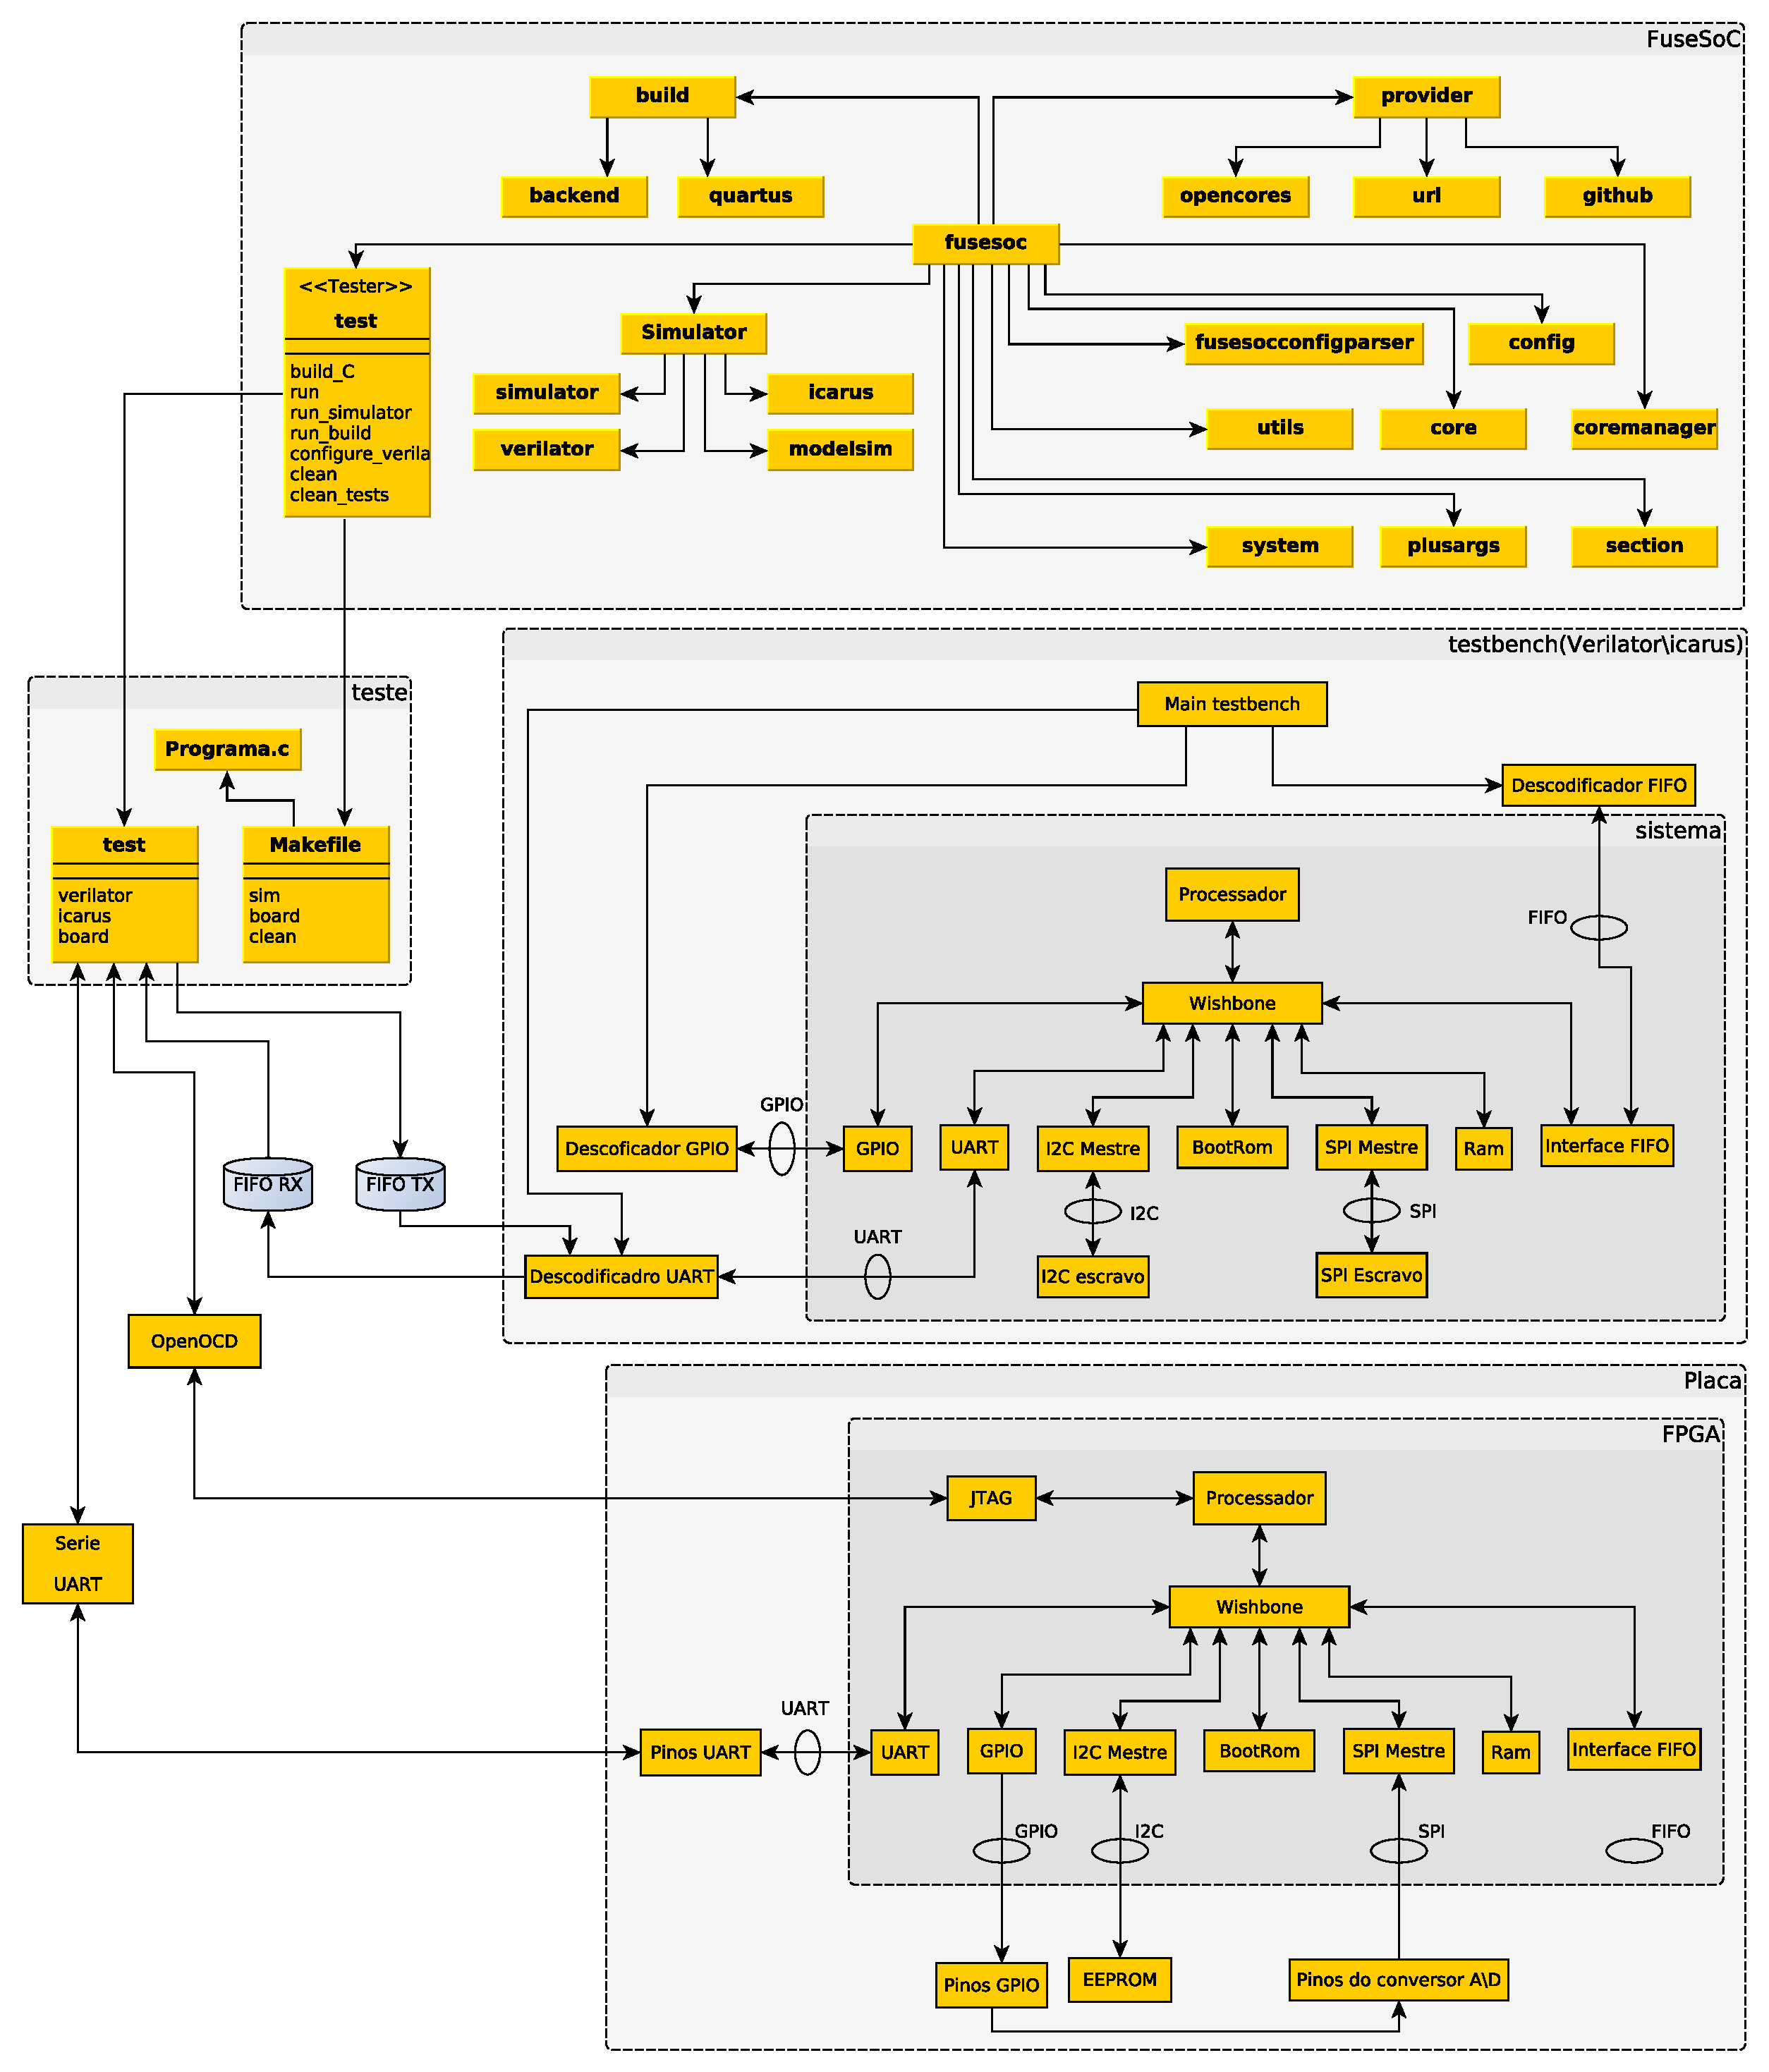
\includegraphics[width=1.00\textwidth]{grafos/Fusesoc_teste.pdf}
  \caption[Diagrama de da plataforma de testes usando o Fusesoc]{Diagrama da plataforma de testes usando o Fusesoc.}
  \label{fig:fusesoc_teste}
\end{figure}


falar sobre as flags do teste
\begin{table}[h!]
  \begin{center}
    \begin{tabular}{|c|C{8cm}|c|}
      \hline
      parametro & Descrição & Default \\
      \hline \hline
      --test & Corre apenas o teste indicado & Corre todos os testes existentes na pasta. \\
      \hline
      --mode & Indica com que ferramenta se pretende fazer os testes  (verilator,icarus,board). & Corre os teste com o verilator. \\ 
      \hline
      --folder & Selectionar uma pasta alternativa com os testes, a partir da raiz. & Selectiona a pasta './orpsoc/orpsoc/test/'.\\
      \hline
      system & Selecionar qual dos sistemas se pretende testar. & Parametro obrigatorio.\\
      \hline
    \end{tabular}
  \end{center}
  \caption[Tabela com os parametros existentes na função de correr testes]{Tabela com os parametros existentes na função de correr testes}
  \label{table:Flags}
\end{table}

como posso ver os resultados dos teste

\section{adicionar novos testes}

fazer novos testes.

\section{Testes desenvolvidos}

para mostrar que o sistema funciona corremante foi desenvolvido estes testes 

\subsection{SPI}

explicar como é testado

\subsubsection{simulador verilator}

\subsubsection{Board FPGA}

\subsection{I2C}

explicar como é testado

\subsubsection{simulador verilator}

\subsubsection{Board FPGA}

\subsection{Interface FIFO}

explicar como é testado

\subsubsection{simulador verilator}

\subsubsection{Board FPGA}

\subsection{Bootrom}

explicar como é testado

\subsubsection{simulador verilator}

\subsubsection{Board FPGA}
 %Thesis_Teste

%%%%%%%%%%%%%%%%%%%%%%%%%%%%%%%%%%%%%%%%%%%%%%%%%%%%%%%%%%%%%%%%%%%%%%%%
%                                                                      %
%     File: Thesis_Results.tex                                         %
%     Tex Master: Thesis.tex                                           %
%                                                                      %
%     Author: Carlos A. Rodrigues                                      %
%     Last modified : 21 Jan 2011                                      %
%                                                                      %
%%%%%%%%%%%%%%%%%%%%%%%%%%%%%%%%%%%%%%%%%%%%%%%%%%%%%%%%%%%%%%%%%%%%%%%%

\chapter{Resultados}
\label{chapter:results}


\section{Analise da área utilizado pelo systema}


\section{Analise da frequencia de trabalho do sistema}

\cleardoublepage

 % file "Thesis_Results.tex"

%%%%%%%%%%%%%%%%%%%%%%%%%%%%%%%%%%%%%%%%%%%%%%%%%%%%%%%%%%%%%%%%%%%%%%%%
%                                                                      %
%     File: Thesis_Conclusions.tex                                     %
%     Tex Master: Thesis.tex                                           %
%                                                                      %
%     Author: Andre C. Marta                                           %
%     Last modified :  2 Jul 2015                                      %
%                                                                      %
%%%%%%%%%%%%%%%%%%%%%%%%%%%%%%%%%%%%%%%%%%%%%%%%%%%%%%%%%%%%%%%%%%%%%%%%

\chapter{Conclusions}
\label{chapter:conclusions}

This document presents a research made to understand the state-of-the-art
methods for developing SoCs using open source hardware and software components.

First, a revision of the evolution of RISC ISAs and processors was made,
comparing it to its CISC counterpart. The advantages of using open source RISC
processors to build SoCs were highlighted and carefully explained. Then followed
a description of the RISC-V ISA and some of its main advantages for SoC
development. Next, a brief survey of SoC trends and features was made and the
most pertinent ones were detailed.

With this, four RISC-V processor cores were identified and their features were
discussed in order to select which one would be chosen to start building the
\socname System On Chip. In the end, the size-optimized PicoRV32 core was
selected because it seems to provide the most adequate features to fulfill the
goals in mind for this dissertation project. Afterwards, a description of the
top-level design intended for the \socname System on Chip was made.

The state-of-the-art methods for SoC verification using open source toolchains
are described, as well as the usual development flow of the entire SoC
development process and how the toolchain is used throughout it. The development
environment to be made in this dissertation project is then introduced,
emphasizing the use of an Ethernet interface with the roles usually played by a
JTAG tap in this kind of systems: loading programs and sending bitstreams from
the host computer to the SoC (which may reside in an FPGA), and
remote debugging of programs running on these.

Some preliminary results regarding PicoRV32's deployment on FPGA are shown and
commented.


% ----------------------------------------------------------------------
\section{Achievements}
\label{section:achievements}

The research made so far has showed that the development of RISC-based systems
is more alive than ever, and it will continue to grow in the upcoming IoT
era. The RISC-V open ISA is a promising initiative; for example, startup SiFive
Inc. has already released the world’s first RISC-V based 64-bit quad-core CPU
to support fully featured operating systems like Linux.

The main features of SoCs for IoT purposes have been identified and an early
approach for the top-level design of the \socname System on Chip has been
defined. A preliminary simplistic diagram for the Test program and software
debug has been produced, although some details have yet to be reviewed and
better analyzed. The previous iterations of the project at hand proved to be
useful for understanding how a robust SoC development environment can be built
using open source components, and will serve as an inspiration for the work to
be carried out during the dissertation project.

Some preliminary experiments have been made to assess the resources needed for
FPGA implementation of the PicoRV32 core. The results show that the PicoRV32
core is indeed small and that this CPU architecture is a good contender for the
development of the \socname System on Chip.

\section{Future Work}
\label{section:future}

\subsection{Dissertation Project}

During the upcoming dissertation project, one of the first main focuses will be
to understand how the PicoRV32 architecture is built and how it implements the
RISC-V ISA. It is necessary to understand how peripheral components and
interfaces such as the UART, SPI and Ethernet interface and the memory
controller can be connected to the CPU's pins such that all components in the
\socname System On Chip commuicate well with each other.

Another important aspect that still needs some further study and research is the
GNU RISC-V toolchain, because the are many details regarding it that are not
still well understood, such as how can Newlib and the GCC and clang/LLVM
cross-compilers be used to make the compilation aware of new hardware units,
their clock frequencies, etc. Also, it will be necessary to study better how
GBD's commands work in order to write the debug software to use with the new
Ethernet communication infrastructure.

The makefiles for implementing the development environment will need to be
written as \socname is built, so to follow its progress. Fortunately, the
makefiles provided in PicoRV32's GitHub repository for this matter seem to have
been well structured and may prove useful for the development environment.

The planning of the tasks for the dissertation project is presented in
Table~\ref{table:planning}.
\begin{table}[!htbp]
	\centering
	\caption{Planning of the dissertation project.}
	\label{table:planning}
	\begin{tabular}{p{11cm}c}
		\toprule
		\textbf{Work Planning}                                                                            & \textbf{Scheduling} \\
		\midrule
		Study PicoRV32 RISC-V documentation and PicoRV32's architecture and examples                      & 18/02 - 25/02       \\
		\midrule
		Build the \socname System on Chip writing Verilog code                                            & 26/02 - 26/03       \\
		\midrule
		Study PicoRV32's Makefiles and toolchain documentation                                            & 27/03 - 04/04       \\
		\midrule
		Write Makefiles to implement the verification environment                                         & 05/04 - 12/04       \\
		\midrule
		Create testbench to verify \socname and its components                                            & 13/04 - 20/04       \\
		\midrule
		Develop debug program                                                                             & 21/04 - 18/05       \\
		\midrule
		Verify \socname with RTL simulations                                                              & 19/05 - 26/05       \\
		\midrule
		Verify \socname with FPGA emulation                                                               & 26/05 - 07/06       \\
		\midrule
		Create/use existing software application and debug it                                             & 08/06 - 15/05       \\
		\midrule
		Write the dissertation report                                                                     & 16/06 - 01/07       \\
		\bottomrule 
	\end{tabular}
\end{table}

\subsection{Future perspectives}

In case the \socname System on Chip is successfully built during the
dissertation project, one of the next future projects will be to integrate in it
one or several Versat~\cite{bib:versat} CGRA cores. This opens new
reconfiguration capabilities for SoCs and development possibilities for IoT
applications. CGRAs offer hardware reconfigurability like FPGAs but are less
power hungry, because the infrastructure that connects the hardware blocks that
make up the reconfigurable array in a CGRA is much smaller than in an FPGA. This
is a consequence of CGRA's operation being done a the word level, while the
FPGA's operation is made at the bit level.

% RASCUNHO, IGNORAR
%The Versat cores can be instantiated as peripheral or co-processor units in the \socname System on Chip, which bestows new configuration capabilities for SoC development. On the one hand, CGRAs are, in a sense, like FPGAs because both consist in reconfigurable arrays of several interconnected smaller hardware blocks whose connections can be configured to emulate a desired circuit (or part of it). On the other hand, CGRAs are much smaller and much less power hungry than FPGAs, because the infrastructure that connects the hardware blocks that make up the reconfigurable array in a CGRA is much smaller than in an FPGA. This is because a CGRA's operation is based on a byte (or sereval bytes) level, while the FPGA operates at the bit level.

% RASCUNHO, IGNORAR
%The hardware blocks that make up the reconfigurable array in a CGRA are components like ALUs, multipliers, MULADDs (i.e. a multiplier in series with an accumulator) and memories, which have inputs and outputs with one or more bytes in size. The FPGA's reconfigurable array, is composed of several Configurable Logic Blocks (CLBs), which in turn are composed of several slices, which in turn are composed of a set number of LUTs, flip-flops and multiplexers~\cite{bib:xilinx}. LUTs are of logic gates hard-wired on the FPGA that store the truth table of a desired logic function. Through them, one can implement logic functions with a precision of bits.

Another interesting future work perspective is to convert the \socname System on
Chip on a Network on Chip (NoC), i.e., replace the bus communication
infrastructure and interfaces in the SoC by a network infrastructure based on
Internet communication protocols such as TCP and IP and routing algorithms.
Components will communicate with each other through routers attached to them
inside the chip. It has already been demonstrated in academia (namely,
in~\cite{bib:noc}) that NoC approaches confer great communication upgrades to
SoCs with conventional bus-based infrastructures in nearly all relevant
parameters such as static and dynamic power, area, throughput, latency and
maximum frequency, which validates this future work perspective.

 % file "Thesis_Conclusions.tex"

% ----------------------------------------------------------------------
%  Appendix (optional)
% ----------------------------------------------------------------------
\appendix
\input{Thesis_Appendix} % file "Thesis_Appendix.tex"

% ----------------------------------------------------------------------
%  Bibliography
% ----------------------------------------------------------------------

% Include all references in .bib file, even non-cited ones...
\nocite{*}

% Produces the bibliography section when processed by BibTeX
%
% Bibliography style
% > entries ordered alphabetically
%\bibliographystyle{plain}
% > unsorted with entries appearing in the order in which the citations appear.
%\bibliographystyle{unsrt}
% > entries ordered alphabetically, with first names and names of journals and months abbreviated
%\bibliographystyle{abbrv}
% > entries ordered alphabetically, with reference markers based on authors' initials and publication year
%\bibliographystyle{alpha}
%
% Replacement bibliography styles provided by 'natbib' package
% (plainnat.bst, abbrvnat.bst, unsrtnat.bst )
% > entries ordered alphabetically
\bibliographystyle{plainnat}
% > unsorted with entries appearing in the order in which the citations appear.
%\bibliographystyle{unsrtnat}
% > entries ordered alphabetically, with first names and names of journals and months abbreviated
%\bibliographystyle{abbrvnat}
% > entries ordered alphabetically, with reference markers based on authors' initials and publication year
%\bibliographystyle{alpha}


% External bibliography database file in the BibTeX format
\cleardoublepage
\bibliography{Thesis_bib_DB} % file "Thesis_bib_DB.bib"
% Add entry in the table of contents as chapter
\addcontentsline{toc}{chapter}{\bibname}
\cleardoublepage

% ----------------------------------------------------------------------
\end{document}
% ----------------------------------------------------------------------

